% latex-beamer, texlive-publishers, texlive-latex-extra
% pdf-presenter-console daetools-introduction.pdf

\documentclass{beamer}
\usepackage{hyperref}
\usepackage[utf8]{inputenc}
\usepackage[english,serbian]{babel}
\usepackage{color}

\usetheme{Luebeck}
\usecolortheme{default}
\usefonttheme{professionalfonts}
\usefonttheme[onlymath]{serif}

%\setbeameroption{show notes}
%\setbeamertemplate{note page}[plain]
\setbeamertemplate{blocks}[rounded][shadow=true]

\definecolor{light_red}{RGB}{255, 100, 100}
\definecolor{light_green}{RGB}{100, 255, 100}

\begin{document}

\title[\textbf{DAE Tools} - Introduction]{\textbf{DAE Tools}: An equation-oriented process\linebreak modelling and optimization software}
\subtitle{\textbf{Introduction}}
\author{Dragan Nikolić}
\institute
{
  DAE Tools Project, \url{http://www.daetools.com}
}
%\logo{\includegraphics{../images/[d][a][e]_Tools_project.png}}
\date{1 December 2013} 
\titlegraphic{\includegraphics{../[d][a][e]_Tools_project.png}}

\AtBeginSection[]
{
  \begin{frame}
    \frametitle{Outline}
    \tableofcontents[currentsection]
  \end{frame}
}

\begin{frame}
\titlepage
\end{frame}

\begin{frame}
\frametitle{Outline}
\tableofcontents[currentsubsection, 
                 hideothersubsections, 
                 sectionstyle=show, 
                 subsectionstyle=hide]
\end{frame} 


\section{Intro}

\subsection{General Info}
\begin{frame}
\frametitle{What is DAE Tools?} 
\begin{block}{}
\begin{itemize}
  \item Process modelling, simulation, optimization and parameter estimation software (www.daetools.com)
  \item Areas of application:
    \begin{itemize}
      \item Initially: chemical process industry (mass, heat and momentum transfers, chemical reactions, separation processes, phase-equilibrium, thermodynamics)
      \item Nowadays: multi-domain
    \end{itemize}
  \item Hybrid approach between general-purpose programming languages (c++, Fortran, Java) and domain-specific modelling languages (Modelica, gPROMS...)
\end{itemize}
\end{block}
\end{frame}

\begin{frame}
\frametitle{What can be done with DAE Tools?} 
\begin{block}{}
\begin{itemize}
  \item Simulation
    \begin{itemize}
      \item Steady-State 
      \item Transient
    \end{itemize}
  \item Optimization
    \begin{itemize}
      \item NLP problems: IPOPT, NLOPT, OpenOpt, scipy.optimize
      \item MINLP problems: BONMIN
    \end{itemize}
  \item Parameter estimation: Levenberg–Marquardt algorithm (scipy.optimize)
\end{itemize}
\end{block}
\end{frame}

\begin{frame}
\frametitle{Types of systems that can be modelled}
\begin{block}{}
\begin{itemize}
  \item Initial value problems of implicit form: systems of linear, non-linear, and (partial-)differential algebraic equations
  \item Index-1 DAE systems
  \item With lumped or distributed parameters: Finite Difference or Finite Elements Methods
  \item Steady-state or dynamic
  \item Continuous with some elements of event-driven systems (discontinuous equations, state transition networks and discrete events) 
\end{itemize}
\end{block}
\end{frame}

\subsection{Motivation}
\begin{frame}
\frametitle{Why yet another software?}
\begin{block}{}
Advantages:
\begin{enumerate}
  \item Hybrid approach betwen DSL and GPPL
  \item Programmatical generation of models
  \item Runtime modification of objcts/models (operating procedures)
  \item Introperability with 3rd party software packages/libraries
  \item Code generation/Model exchange capabilities
\end{enumerate}
\end{block}
\end{frame}

\subsection{Main features}
\begin{frame}
\frametitle{Not a modelling language}
\begin{block}{}
\begin{itemize}
  \item A set of software packages
  \item API for:
  \begin{itemize}
    \item Model development
    \item Results processing (plotting, various file formats)
    \item Simulation, optimization and parameter estimation
    \item Code generation for other DSLs and programming languages
    \item Report generation (XML+MathML) and model exchange
  \end{itemize}
  \item Large set of supported solvers (DAE, LA, NLP, MINLP)
\end{itemize}
\end{block}
\end{frame}

\begin{frame}
\frametitle{Not a modelling language (cont'd)}
\begin{block}{}
\begin{itemize}
  \item Allows easy interaction with other software libraries 
        (two-way interoperability with other software, embedding in other software etc.)
  \item Free/Open source software (GNU GPL)
  \item Cross-platform (GNU/Linux, MacOS, Windows)
  \item Supports multiple architectures (32/64 bit x86, arm, any other with the GNU toolchain)
  \item Developed in c++ with Python bindings (Boost.Python)
\end{itemize}
\end{block}
\end{frame}

\begin{frame}
\frametitle{Object-oriented modelling}
\begin{block}{}
\begin{itemize}
  \item Everything is an object (models, parameters, variables, equations, state transition networks, simulations, solvers, ...) 
  \item Models are classes derived from the base daeModel class (inheriting the common functionality)
  \item Hierarchical model decomposition allows creation of complex, re-usable model definitions
  \item All Object Oriented concepts supported (such as multiple inheritance, templates, polymorphism, ...) 
        that are supported by the target language (c++, Python), except:
  \begin{itemize}
      \item Derived classes always inherit all declared objects (parameters, variables, equations, ...)  
      \item All parameters, variables, equations etc. remain public
  \end{itemize}
\end{itemize}
\end{block}
\end{frame}

\begin{frame}
\frametitle{Equation-oriented (acausal) modelling}
\begin{block}{}
\begin{itemize}
  \item Equations given in an implicit form (as a residual)
    \begin{center}
      $F(\dot {x}, x, y, p) = 0$
    \end{center}
  \item Input-Output causality is not fixed:
  \begin{itemize}
    \item Increased model re-use
    \item Support for different simulation scenarios (based on a single model) by specifying different degrees of freedom
  \end{itemize}
  \item For instance, equation given in the following form:
    \begin{center}
      $x_1 + x_2 + x_3 = 0$
    \end{center}
    can be used to determine either $x_1$, $x_2$ or $x_3$ depending on what combination of variables is known:
    \begin{center}
      $x_1 = -x_2 - x_3 \; or \;  
      x_2 = -x_1 - x_3 \; or \; 
      x_3 = -x_1 - x_2$
    \end{center}
\end{itemize}
\end{block}
\end{frame}

\begin{frame}
\frametitle{Separation of models definition from operations on them}
\begin{block}{}
\begin{itemize}
  \item The structure of the model (parameters, variables, equations etc.) given in the model classes ($daeModel$, $daeFiniteElementModel$) 
  \item The runtime information in the simulation class ($daeSimulation$)
  \item Single model definition, but:
  \begin{itemize}
    \item One or more different simulation scenarios
    \item One or more optimization scenarios
  \end{itemize}
\end{itemize}
\end{block}
\end{frame}

\begin{frame}
\frametitle{Hybrid continuous/discrete systems}
\begin{block}{}
\begin{itemize}
  \item Modelling of continuous systems with some elements of event-driven systems 
  \begin{itemize}
    \item Discontinuous equations
    \item State transition networks
    \item Discrete events
  \end{itemize}
\end{itemize}
\end{block}
\end{frame}

\begin{frame}
\frametitle{Code generation}
\begin{block}{}
\begin{itemize}
  \item Model export from DAE Tools to other DSL/modelling/programming languages
  \begin{itemize}
    \item Modelica
    \item c99
  \end{itemize}
\end{itemize}
\end{block}
\end{frame}

\begin{frame}
\frametitle{Model Exchange}
\begin{block}{}
\begin{itemize}
  \item Support for Functional Mock-up Interface for Model Exchange and Co-Simulation (FMI): https://www.fmi-standard.org 
  \item FMI – a tool independent standard to support both model exchange and co-simulation of dynamic models using a combination of xml-files and compiled C-code
  \item Still in experimental phase
\end{itemize}
\end{block}
\end{frame}

\begin{frame}
\frametitle{Model reports}
\begin{block}{}
\begin{itemize}
  \item Automatic model documentation
  \item XML + MathML format
  \item XSL transformation used to to generate HTML code and visualize reports 
  \item Two types:
  \begin{itemize}
    \item Model description report (contains model definition)
    \item Runtime report with all values and equations expanded (contains definition of the simulation)
  \end{itemize}
\end{itemize}
\end{block}
\end{frame}

\begin{frame}
\frametitle{Model reports (cont'd)}
\includegraphics<1>[height=0.7\paperheight]{../_static/model_report.png}
\includegraphics<2>[height=0.7\paperheight]{../_static/runtime_model_report.png}
\end{frame}

\begin{frame}
\frametitle{Multi-domain}
\begin{block}{}
\begin{itemize}
  \item From chemical processing industry to biological neural networks
  \item DAE Tools is not a DSL but defines the basic modelling concepts such as models, parameters, variables, various types of equations 
        (ordinary, differential, partial differential, discontinuous), state transition networks etc. that can be used as building blocks 
        for a specific domain
  \item Example: a reference implementation simulator for NineML (xml-based modelling language for describing networks of spiking neurons)
  \item The key concepts from NineML are based on DAE Tools concepts: Neurone, Synapse, Population of neurones, Layers, Projections etc
\end{itemize}
\end{block}
\end{frame}

\begin{frame}
\frametitle{DAE Plotter}
\begin{columns}
  \begin{column}{0.5\paperwidth}
    \begin{center}
      \begin{itemize}
	\item 2D plots (Matplotlib)
	\item Animated 2D plots
	\item 3D plots (Mayavi)
      \end{itemize}
    \end{center}
    \begin{center}
      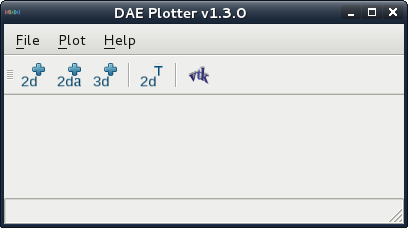
\includegraphics[width=0.35\paperwidth]{../_static/daeplotter.png}
    \end{center}
  \end{column}
  \begin{column}{0.5\paperwidth}
    \begin{center}
      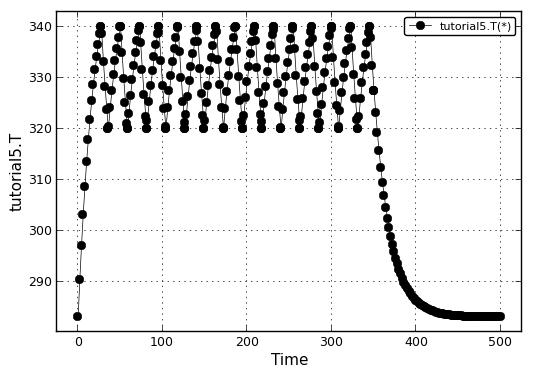
\includegraphics[width=0.35\paperwidth]{../_static/sample_2d_plot.png}
    \end{center}
    \begin{center}
      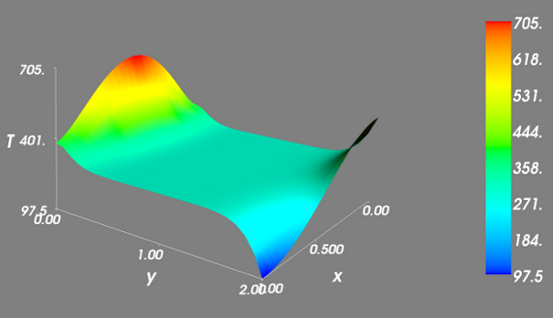
\includegraphics[width=0.3\paperwidth]{../_static/sample_3d_plot.png}
    \end{center}
  \end{column}
\end{columns}
\end{frame}

\begin{frame}
\frametitle{Solvers}
\begin{block}{}
Supported DAE solvers@
\begin{itemize}
  \item Sundials IDAS ({\small https://computation.llnl.gov/casc/sundials/main.html})
\end{itemize}
\end{block}

\begin{block}{}
Supported FE libraries:
\begin{itemize}
  \item deal.II ({\small http://dealii.org})
\end{itemize}
\end{block}

\begin{block}{}
Supported optimization solvers:
\begin{itemize}
  \item IPOPT ({\small https://projects.coin-or.org/Ipopt}) 
  \item Bonmin ({\small https://projects.coin-or.org/Bonmin}) 
  \item NLOPT ({\small http://ab-initio.mit.edu/wiki/index.php/NLopt}) 
\end{itemize}
\end{block}
\end{frame}

\begin{frame}
\frametitle{Solvers}
\begin{block}{}
Supported LA solvers:
\begin{itemize}
  \item Sundials dense LU, Lapack
  \item Trilinos Amesos ({\small http://trilinos.sandia.gov/packages/amesos}) 
  \item Trilinos AztecOO ({\small http://trilinos.sandia.gov/packages/aztecoo}) 
  \item SuperLU SuperLU-MT ({\small http://crd.lbl.gov/~xiaoye/SuperLU/index.html}) 
  \item Umfpack ({\small http://www.cise.ufl.edu/research/sparse/umfpack}) 
  \item MUMPS ({\small http://graal.ens-lyon.fr/MUMPS})
  \item CUSP ({\small http://code.google.com/p/cusp-library}) 
  \item Intel Pardiso ({\small http://software.intel.com/en-us/articles/intel-mkl})
\end{itemize}
\end{block}
\end{frame}



\section{Programming paradigms}

\subsection{General}
\begin{frame}
\frametitle{Approaches to process modelling}
\begin{block}{}
\begin{itemize}
  \item Two approaches to process modelling:
  \begin{itemize}
    \item Domain Specific Language (DSL)
    \item General-purpose programming language (such as c, c++, Java or Python)
  \end{itemize}
\end{itemize}
\end{block}
\end{frame}

\begin{frame}
\frametitle{Domain Specific Languages}
\begin{block}{}
\begin{itemize}
  \item Special-purpose programming or specification languages dedicated to a particular problem domain
  \item Designed to directly support the key concepts from that domain
  \item Specifically created to solve problems in a particular domain
  \item (Usually) not intended to solve problems outside that domain (although that may be technically possible in some cases)
  \item Commonly lack low-level functions for filesystem access, interprocess control, and other functions that characterize 
	full-featured programming languages, scripting or otherwise
  \item Examples: Modelica, gPROMS, SpeedUp, Ascend, GAMS ...
\end{itemize}
\end{block}
\end{frame}

\begin{frame}
\frametitle{General-purpose programming languages}
\begin{block}{}
\begin{itemize}
  \item Created to solve problems in a wide variety of application domains
  \item Do not support key concepts from any domain
  \item Have low-level functions for filesystem access, interprocess control etc.
  \item Examples: c, c++, Fortran, Python, Java etc.
  \item Typical scenario: solving a DAE system
  \begin{itemize}
    \item Choose a solver (Sundials IDA, DASSL, RADAU5, DAEPACK etc)
    \item Implement user functions to manually calculate residuals and derivatives for a Jacobian matrix, apply boundary conditions etc
    \item Create an executable program
  \end{itemize}
\end{itemize}
\end{block}
\end{frame}

\begin{frame}
\frametitle{DAE Tools approach}
\begin{block}{}
A sort of the hybrid approach:
\begin{itemize}
  \item Applies general-purpose programming languages such as c++ and Python
  \item Offers a class-hierarchy/API that resembles a syntax of a DSL as much as possible. 
  \item Provides low-level concepts such as parameters, variables, equations, ports, models, state transition networks, discrete events etc.
  \item Concepts from new application domains can be added on top of its low level concepts (for instance the simulator for biological neural networks - NineML, as it will be shown later in Use Case section)
  \item Enables an access to the low-level functions and a large number of standard libraries
  \item Enables access to a large number of state-of-the-art scientific libraries (either free/open-source or proprietary)
\end{itemize}
\end{block}
\end{frame}

\subsection{DSL vs. DAE Tools}
\begin{frame}
\frametitle{gPROMS vs. Modelica}
\begin{columns}[b]
  \begin{column}{0.5\paperwidth}
    \begin{center}
      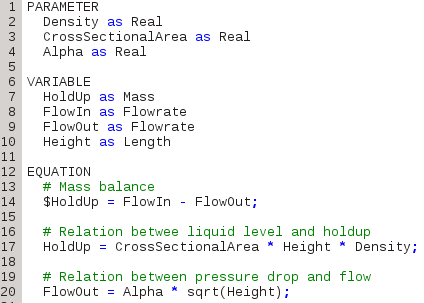
\includegraphics[width=0.45\paperwidth]{../_static/gPROMS_model.png}
    \end{center}
    \begin{center}
      {\small Model developed in gPROMS\\
	      http://www.psenterprise.com}
    \end{center}
  \end{column}
  \begin{column}{0.5\paperwidth}
    \begin{center}
      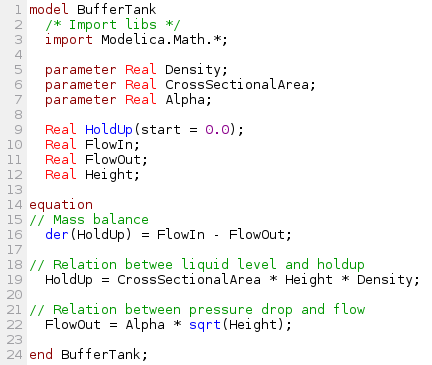
\includegraphics[width=0.45\paperwidth]{../_static/modelica_model.png}
    \end{center}
    \begin{center}
      {\small The same model in OpenModelica\\
	      https://www.openmodelica.org}
    \end{center}
  \end{column}
\end{columns}
\end{frame}

\begin{frame}
\frametitle{DAE Tools}
  \begin{center}
    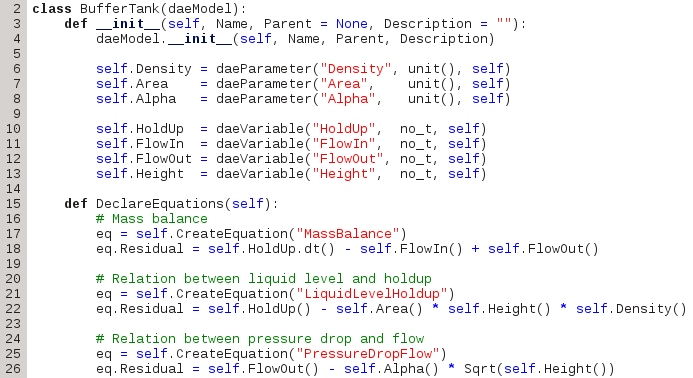
\includegraphics[width=0.85\paperwidth]{../_static/daetools_model.png}
  \end{center}
  \begin{center}
    {\small The same model in daetools}
  \end{center}
\end{frame}

\begin{frame}
\frametitle{Key modelling concepts \& grammar}
\begin{block}{\textcolor{light_green}{DSL/Modelling languages}}
\begin{itemize}
  \item Domain-specific languages allow solutions to be expressed in the idiom and at the level of abstraction of the problem domain 
        (direct support for all modelling concepts by the language syntax)
\end{itemize}
\end{block}

\begin{block}{\textcolor{light_red}{DAE Tools}}
\begin{itemize}
  \item Modelling concepts cannot be expressed directly in the programming language and have to be emulated in the API or in 
        some other way
\end{itemize}
\end{block}
\end{frame}

\begin{frame}
\frametitle{Verbosity}
\begin{block}{\textcolor{light_green}{DSL/Modelling languages}}
\begin{itemize}
  \item Clean, concise, ellegant and natural way of building model descriptions: the code can be self documenting
\end{itemize}
\end{block}

\begin{block}{\textcolor{light_red}{DAE Tools}}
\begin{itemize}
  \item The support for modelling concepts is much more verbose and less elegant; however, DAE Tools can generate XML+MathML
	based model reports that can be either rendered in XHTML format using XSLT transformations (representing the code documentation)
	or used as an XML-based model exchange language
\end{itemize}
\end{block}
\end{frame}

\begin{frame}
\frametitle{Maintainability \& portability}
\begin{block}{\textcolor{light_green}{DSL/Modelling languages}}
\begin{itemize}
  \item Domain-specific languages could enhance quality, productivity, reliability, maintainability and portability
\end{itemize}
\end{block}

\begin{block}{\textcolor{light_red}{DAE Tools}}
\begin{itemize}
  \item 
\end{itemize}
\end{block}
\end{frame}

\begin{frame}
\frametitle{Simulators \& programming languages}
\begin{block}{\textcolor{light_green}{DSL/Modelling languages}}
\begin{itemize}
  \item DSLs could be and often are simulator independent making a model exchange easier
\end{itemize}
\end{block}

\begin{block}{\textcolor{light_red}{DAE Tools}}
\begin{itemize}
  \item Programming language dependent; however, a large number of scientific software libraries exposes its functionality
        to Python via Python wrappers
\end{itemize}
\end{block}
\end{frame}

\begin{frame}
\frametitle{Need for a compiler/parser/interpreter}
\begin{block}{\textcolor{light_red}{DSL/Modelling languages}}
\begin{itemize}
  \item Cost of designing, implementing, and maintaining a domain-specific language as well as the tools required to develop with it (IDE):
        a compiler/lexical parser/interpreter must be developed with all burden that comes with it (such as error handling, grammar ambiguities,
        hidden bugs etc)
\end{itemize}
\end{block}

\begin{block}{\textcolor{light_green}{DAE Tools}}
\begin{itemize}
  \item A compiler/lexical parser/interpreter is an integral part of the programming language (c++, Python) with a robust error handling,
        universal grammar and massively tested
\end{itemize}
\end{block}
\end{frame}

\begin{frame}
\frametitle{Need for a new language syntax}
\begin{block}{\textcolor{light_red}{DSL/Modelling languages}}
\begin{itemize}
  \item Cost of learning a new language vs. its limited applicability: users are required to master a new language
        (yet another language grammar)
\end{itemize}
\end{block}

\begin{block}{\textcolor{light_green}{DAE Tools}}
\begin{itemize}
  \item No learning of a new language required (everything can get done in a favourite programming language)
\end{itemize}
\end{block}
\end{frame}

\begin{frame}
\frametitle{Interoperability with the $3^{rd}$ party software}
\begin{block}{\textcolor{light_red}{DSL/Modelling languages}}
\begin{itemize}
  \item Increased difficulty of integrating the DSL with other components: calling external functions/libraries and interaction with
        other software is limited by the existence of wrappers around a simulator engine (for instance some scripting languages like
        Python or javascript)
\end{itemize}
\end{block}

\begin{block}{\textcolor{light_green}{DAE Tools}}
\begin{itemize}
  \item Calling external functions/libraries is a natural and straightforward Interaction with other software is
        natural and straightforward
\end{itemize}
\end{block}
\end{frame}

\begin{frame}
\frametitle{Runtime generation \& modification}
\begin{block}{\textcolor{light_red}{DSL/Modelling languages}}
\begin{itemize}
  \item Models usually cannot be created in the runtime/on the fly (or at least not easily) 
        and cannot be modified in the runtime
\end{itemize}
\end{block}

\begin{block}{\textcolor{light_green}{DAE Tools}}
\begin{itemize}
  \item Models can be created in the runtime/on the fly and easily modified in the runtime
\end{itemize}
\end{block}
\end{frame}

\begin{frame}
\frametitle{Simulation setup}
\begin{block}{\textcolor{light_red}{DSL/Modelling languages}}
\begin{itemize}
  \item Setting up a simulation (ie. the values of parameters values, initial conditions, initially active states)
        is embedded in the language and it is typically difficult to do it on the fly or to obtain the values from some other software
        (for example to chain several software calls where outputs of previous calls represent inputs to the subsequent ones) 
\end{itemize}
\end{block}

\begin{block}{\textcolor{light_green}{DAE Tools}}
\begin{itemize}
  \item Setting up a simulation is done programmaticaly and the initial values can be obtained from some other software in a natural way
        (chaining several software calls is easy since a large number of libraries make Python wrappers available)
\end{itemize}
\end{block}
\end{frame}

\begin{frame}
\frametitle{Operating procedures}
\begin{block}{\textcolor{light_red}{DSL/Modelling languages}}
\begin{itemize}
  \item Simulation operating procedures are not flexible; manipulation of model parameters, variables, equations, simulation results
        etc is limited to only those operations provided by the language 
\end{itemize}
\end{block}

\begin{block}{\textcolor{light_green}{DAE Tools}}
\begin{itemize}
  \item Operating procedures are completely flexible (within the limits of a programming language itself)
        and a manipulation of model parameters, variables, equations, simulation results etc can be done in any way which
        a user cosiders suitable for his/her problem 
\end{itemize}
\end{block}
\end{frame}

\begin{frame}
\frametitle{Outputs}
\begin{block}{\textcolor{light_red}{DSL/Modelling languages}}
\begin{itemize}
  \item Only the type of results provided by the language/simulator is available; custom processing is usually not possible or
        if a simulator does provide a way to build extensions it is limited to the functionality made available to them 
\end{itemize}
\end{block}

\begin{block}{\textcolor{light_green}{DAE Tools}}
\begin{itemize}
  \item The results processing can be done in any way which a user considers suitable(again within the limits
        of a programming language itself) 
\end{itemize}
\end{block}
\end{frame}

\section{Architecture}

\subsection{Overview}
\begin{frame}
\frametitle{Available modules}
\begin{block}{}
\begin{itemize}
  \item pyDAE:
  \begin{itemize}
    \item pyCore (key modelling concepts)
    \item pyActivity (simulation, optimization)
    \item pyDataReporting (results handling)
    \item pyIDAS (DAE solver)
    \item pyUnits ($unit$ and $quantity$ concepts)
  \end{itemize}
\end{itemize}
\end{block}
\begin{block}{}
\begin{itemize}
  \item FE Solvers: 
  \begin{itemize}
    \item pyDealII
  \end{itemize}
\end{itemize}
\end{block}
\end{frame}

\begin{frame}
\frametitle{Available modules (cont'd)}
\begin{block}{}
\begin{itemize}
  \item LA Solvers: 
  \begin{itemize}
    \item pySuperLU
    \item pySuperLU\_MT
    \item pyTrilinos (Amesos, AztecOO)
    \item pyIntelPardiso
  \end{itemize}
\end{itemize}
\end{block}
\begin{block}{}
\begin{itemize}
  \item NLP/MINLP Solvers: 
  \begin{itemize}
    \item pyIPOPT
    \item pyBONMIN
    \item pyNLOPT
  \end{itemize}
\end{itemize}
\end{block}
\end{frame}

\begin{frame}
\frametitle{Available components}
\begin{block}{}
\begin{itemize}
  \item Model
  \item Simulation
  \item Optimization
  \item DAE solver
  \item LA solver
  \item NLP solver
  \item Log
  \item Data reporter
  \item Data receiver
\end{itemize}
\end{block}
\end{frame}

\begin{frame}
\frametitle{Available components (cont'd)}
\begin{center}
  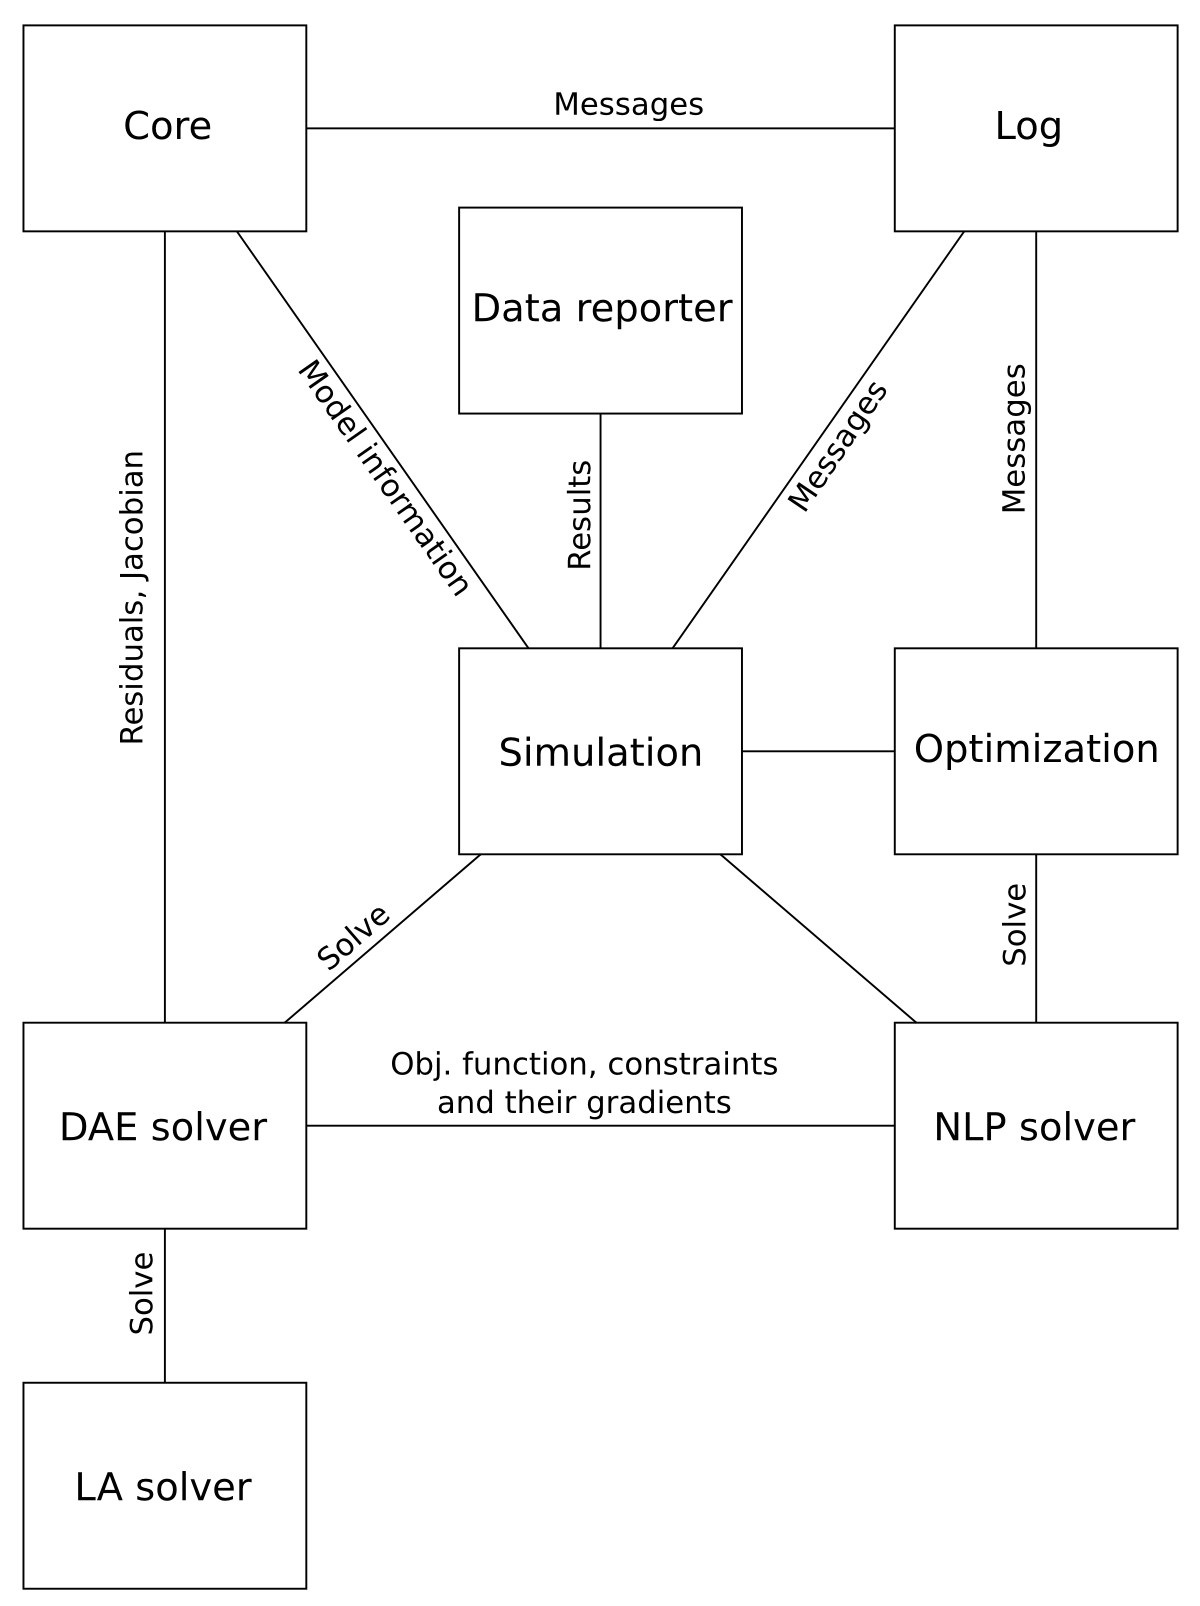
\includegraphics[height=0.7\paperheight]{../_static/daetools-architecture.png}
\end{center}
\end{frame}

\section{Use Cases} 

\subsection{Use Case 1 - High level modelling language}
\begin{frame}
\frametitle{}
\end{frame}

\subsection{Use Case 2 - Low level DAE solver}
\begin{frame}
\frametitle{}
\end{frame}

\subsection{Use Case 3 - Embedded simulator (back end)}
\begin{frame}
\frametitle{}
\end{frame}

\end{document}